\documentclass[margin=10pt,border=2mm,11pt]{standalone}
\usepackage{tikz}
\usepackage{times}
\usepackage{xcolor}
\usetikzlibrary{shapes.misc,calc,arrows,arrows.meta,patterns}

\definecolor{red1}{HTML}{E07A5F}
\definecolor{blue1}{HTML}{3D405B}
\definecolor{green1}{HTML}{81B29A}
\definecolor{orange1}{HTML}{F2CC8F}
\definecolor{tan1}{HTML}{F4F1DE}
\definecolor{brightorange1}{HTML}{FCA311}

\newcommand{\cmark}{\ding{51}}%
\newcommand{\xmark}{\ding{55}}%
\newcommand{\smin}{\scalebox{0.9}[0.6]{-}}
\newcommand{\A}{\mathcal{A}}

\begin{document}


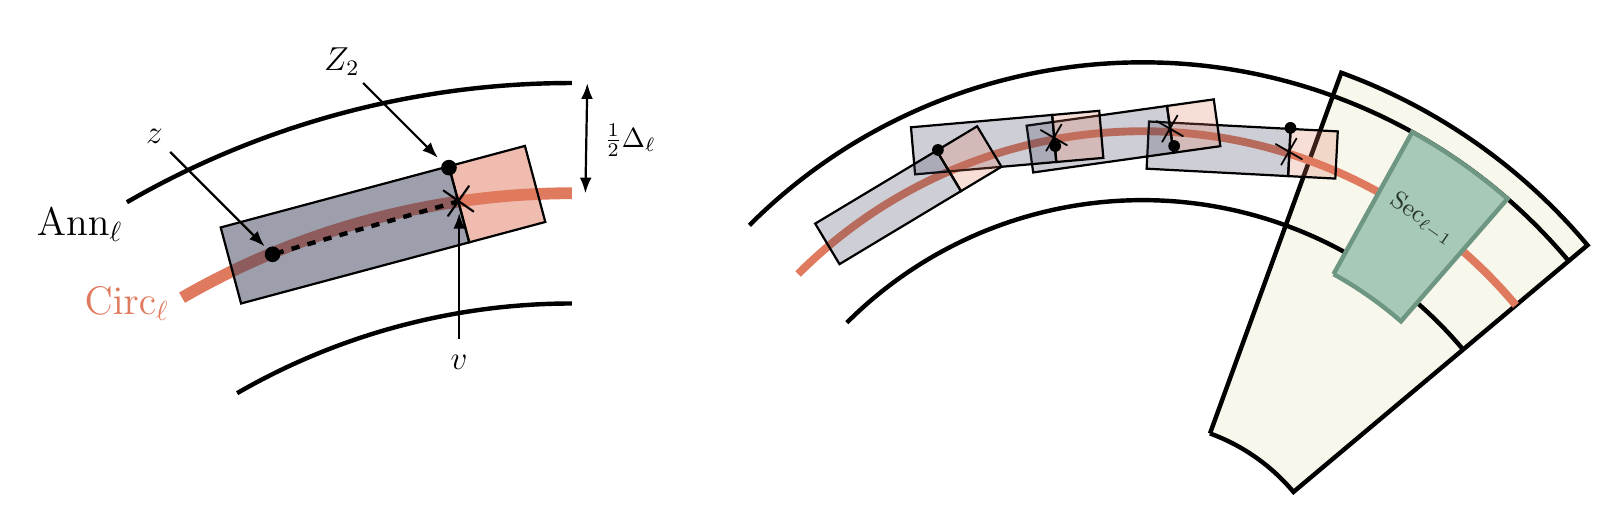
\begin{tikzpicture}

\begin{scope}[shift={(0,0)}]

\begin{scope}[scale=2,shift={(3,-2.25)},rotate=0]
\draw[ultra thick] (105+15:5.5+0.15) arc (105+15:75+15:5.5+0.15);
\draw[line width=1.5mm,color=red1] (105+15:4.95) arc (105+15:75+15:4.95);
\draw[ultra thick] (105+15:4.25) arc (105+15:75+15:4.25);
\draw[thick,{Latex[length=2mm]}-{Latex[length=2mm]}] (75+14:4.95) -- (75+14:5.5+0.15);
\node at (75+11:5.3) {$\frac12 \Delta_\ell$};
\end{scope}



\begin{scope}[scale=2,shift={(0.9,2)},rotate=15]
\draw[thick,fill=red1,fill opacity=0.5] (1.5,0) rectangle (2,0.5);
\draw[thick,fill=blue1,fill opacity=0.5] (0,0) rectangle (1.5,0.5);
\end{scope}


\node at (4.35-1.27,5.8+1.27) {\large $Z_{2}$};
\draw[thick,-{Latex[length=2mm]}] (4.35-1,5.8+1) -- (4.35-0.05,5.8+0.05);
\node at (4.44,5.725)[circle, fill=black, inner sep=2pt]{};
\node at (2.2,4.625)[circle, fill=black, inner sep=2pt]{};
\draw[thick,-{Latex[length=2mm]}] (2.2-1.3,4.625+1.3) -- (2.2-0.1,4.625+0.1);
\node at (2.2-1.5,4.625+1.5) {\large $z$};

\node[color=black,rotate=10] at (4.57,5.8-0.5) {\huge $\times$};
\draw[thick,-{Latex[length=2mm]}] (4.57,5.8-2.25) -- (4.57,5.8-0.5-0.15);
\node at (4.57,5.8-2.55) {\large $v$};

\node at (-.25,5) {\Large $\mathrm{Ann}_\ell$};
\node[color=red1] at (0.35,4) {\Large $\mathrm{Circ}_\ell$};

\draw[dashed,ultra thick] (4.57,5.8-0.5) -- (2.2,4.625);

\end{scope}

\begin{scope}[scale=1,shift={(7,0)}]

\begin{scope}[scale=1.25,shift={(5,0)},rotate=0]
\draw[ultra thick,fill=tan1!60] (55+15:2) -- (55+15:5.9) arc (55+15:55-15:5.9) -- (55-15:2) arc (55-15:55+15:2);
\draw[ultra thick] (120+15:5.5+0.15) arc (120+15:40:5.5+0.15);
\draw[line width=1mm,color=red1] (120+15:4.95) arc (120+15:40:4.95);
\draw[ultra thick] (120+15:4.25) arc (120+15:40:4.25);
\draw[ultra thick,color=green1!85!black,fill=green1!70] (55+6:4.) -- (55+6:5.65) arc (55+6:55-6:5.65) -- (55-6:4) arc (55-6:55+6:4);
\node[color=green1!30!black,rotate=-35] at (55:4.95) {\small $\mathrm{Sec}_{\ell{-}1}$};
\end{scope}


\begin{scope}[scale=1.2,shift={(5.25,4.76)},rotate=-3]
\draw[thick,fill=red1,fill opacity=0.25] (1.5,0) rectangle (2,0.5);
\draw[thick,fill=blue1,fill opacity=0.25] (0,0) rectangle (1.5,0.5);
\node[color=black,rotate=15] at (1.5,0.25) {\LARGE $\times$};
\end{scope}


\begin{scope}[scale=1.2,shift={(4.05,4.72)},rotate=8]
\draw[thick,fill=red1,fill opacity=0.25] (1.5,0) rectangle (2,0.5);
\draw[thick,fill=blue1,fill opacity=0.25] (0,0) rectangle (1.5,0.5);
\node[color=black,rotate=15] at (1.5,0.25) {\LARGE $\times$};
\end{scope}


\begin{scope}[scale=1.2,shift={(2.8,4.7)},rotate=5]
\draw[thick,fill=red1,fill opacity=0.25] (1.5,0) rectangle (2,0.5);
\draw[thick,fill=blue1,fill opacity=0.25] (0,0) rectangle (1.5,0.5);
\node[color=black,rotate=15] at (1.5,0.25) {\LARGE $\times$};
\end{scope}

\begin{scope}[scale=1.2,shift={(2,3.75)},rotate=31]
\draw[thick,fill=red1,fill opacity=0.25] (1.5,0) rectangle (2,0.5);
\draw[thick,fill=blue1,fill opacity=0.25] (0,0) rectangle (1.5,0.5);

\end{scope}



\node at (3.65,5.95)[circle, fill=black, inner sep=1.5pt]{};
\node at (5.14,6)[circle, fill=black, inner sep=1.5pt]{};
\node at (6.65,6)[circle, fill=black, inner sep=1.5pt]{};
\node at (8.127,6.23)[circle, fill=black, inner sep=1.5pt]{};
\end{scope}

\end{tikzpicture}


\end{document}